\q{11}{Preprocessing Bayes' Nets for Inference}

\begin{tabular}{ll}
\begin{minipage}{0.7\textwidth}
For (a) and (b), consider the Bayes' net shown on the right.  You are given
the structure but you are not given the
conditional probability tables (CPTs).  We will consider the query $P(B|D = True)$,
and reason about which steps in the variable elimination process we might be able
to execute based on just knowing the graph structure and not the CPTs.
\end{minipage}
&
\begin{minipage}{0.25\textwidth}
\centering
    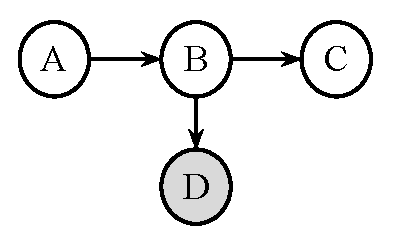
\includegraphics[width=0.8\textwidth]{figs/elimination1.pdf}
\end{minipage}
\\
\end{tabular}
\begin{question}{[1 pt]}
Assume the first variable we want to eliminate is $A$ and the
resulting factor would be $f_1(B)$. Can $f_1(B)$ be computed from what we are given? If so, what are its values?\\
\vspace{1.4cm} \textbf{We cannot compute $f_1(B)$}
\end{question}

\begin{question}{[1 pt]}
Assume the first variable we eliminate is $C$ and the resulting factor is $g_1(B)$. Can $g_1(B)$ be computed from what we are given? If so, what are its values?\\
\vspace{1.4cm} $g_1(B=0)=0.5$ and $g_1(B=1)=0.5$
\end{question}

\begin{tabular}{ll}
\begin{minipage}{0.7\textwidth}
For (c) through (g),  consider the Bayes' net shown on the right.  You are given
the structure but you are not given the
conditional probability tables (CPTs).  We will consider the query $P(B|G = True)$,
and again we will reason about which steps in the variable elimination process we might be able
to execute based on just knowing the graph structure and not the CPTs.
\end{minipage}
&
\begin{minipage}{0.25\textwidth}
\centering
    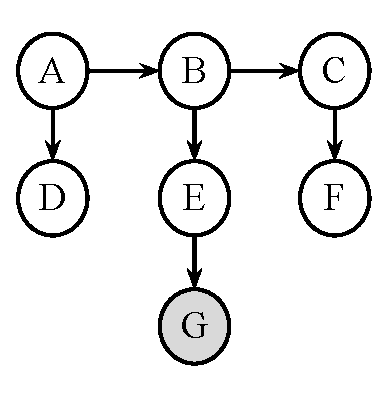
\includegraphics[width=0.6\textwidth]{figs/elimination2.pdf}
\end{minipage}
\\
\end{tabular}

\begin{question}{[1 pt]}
Assume the first variable we eliminate is $D$ and the resulting factor is $h_1(A)$. Can $h_1(A)$ be computed from what we are given? If so, what are its values?\\
\vspace{1.4cm} $h_1(A=0)=0.5$ and $h_1(A=1)=0.5$
\end{question}

\begin{question}{[1 pt]}
Assume the first 2 variables we eliminate are $A$ and $D$ and the resulting factor is $i_2(B)$. Can $i_2(B)$ be computed from what we are given? If so, what are its values?\\
\vspace{1.4cm} \textbf{We cannot compute $i_2(B)$}
\end{question}

\begin{question}{[1 pt]}
Assume the first variable we eliminate is $F$ and the resulting factor is $j_1(C)$. Can $i_2(B)$ be computed from what we are given? If so, what are its values?\\
\vspace{1.4cm} $j_1(C=0)=0.5$ and $j_1(C=1)=0.5$
\end{question}

\begin{question}{[1 pt]}
Assume the first 2 variables we eliminate are $F$and $C$ and the resulting factor is $k_2(B)$. Can $k_2(B)$ be computed from what we are given? If so, what are its values?\\
\vspace{1.4cm} $k_2(B=0)=0.5$ and $k_2(B=1)=0.5$
\end{question}

\begin{question}{[1 pt]}
Assume the first variable we eliminate is $E$ and the resulting factor is $l_1(B,G = True)$. Can $l_1(B, G = True)$ be computed from what we are given? If so, what are its values?\\
\textbf{We cannot compute $l_1(B,+g)$}
\end{question}

{\newpage}
\begin{question}{[4 pts]}
In the smaller examples in (a) through (g) you will have observed that
sometimes a variable can be eliminated without knowing any of the CPTs.
This means that variable's CPT does not affect the answer to the
probabilistic inference query and that variable can be removed from the graph for
the purposes of that probabilistic inference query.  Now consider the following,
larger Bayes' net with the query $P(Q|E = True)$.\\

\centering
    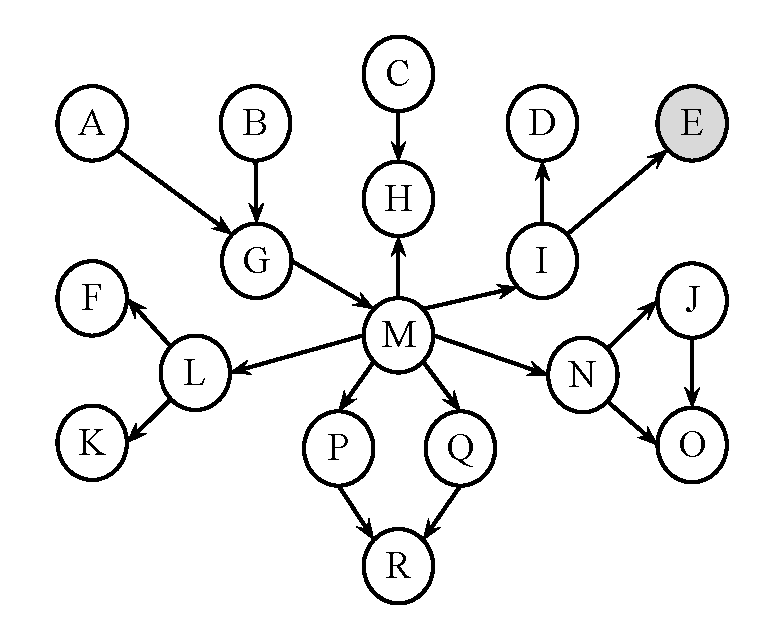
\includegraphics[width=0.5\textwidth]{figs/elimination3.pdf}
\vspace{1cm}
\\Mark all of the variables whose CPTs do \textit{not} affect the value of $P(Q|E = True)$:

% YOUR ANSWER HERE
% You can replace \mcqb with \mcqs
\begin{center}
\begin{tabular}{lllll}
\mcqb $A \phantom{----}$  & \mcqb $B \phantom{----}$  & \mcqb $C \phantom{----}$  & \mcqs $D \phantom{----}$  & \mcqb $E \phantom{----}$   \\ [1em]
\mcqs $F \phantom{----}$  & \mcqb $G \phantom{----}$  & \mcqb $H \phantom{----}$  & \mcqb $I \phantom{----}$  & \mcqs $J \phantom{----}$   \\ [1em]
\mcqs $K \phantom{----}$  & \mcqs $L \phantom{----}$  & \mcqb $M \phantom{----}$  & \mcqs $N \phantom{----}$  & \mcqs $O \phantom{----}$   \\ [1em]
\mcqs $P \phantom{----}$  & \mcqb $Q \phantom{----}$  & \mcqs $R \phantom{----}$ & & \\[1em]
\end{tabular}
\end{center}

\end{question}

